% Options for packages loaded elsewhere
\PassOptionsToPackage{unicode}{hyperref}
\PassOptionsToPackage{hyphens}{url}
%
\documentclass[
]{article}
\usepackage{amsmath,amssymb}
\usepackage{lmodern}
\usepackage{ifxetex,ifluatex}
\ifnum 0\ifxetex 1\fi\ifluatex 1\fi=0 % if pdftex
  \usepackage[T1]{fontenc}
  \usepackage[utf8]{inputenc}
  \usepackage{textcomp} % provide euro and other symbols
\else % if luatex or xetex
  \usepackage{unicode-math}
  \defaultfontfeatures{Scale=MatchLowercase}
  \defaultfontfeatures[\rmfamily]{Ligatures=TeX,Scale=1}
\fi
% Use upquote if available, for straight quotes in verbatim environments
\IfFileExists{upquote.sty}{\usepackage{upquote}}{}
\IfFileExists{microtype.sty}{% use microtype if available
  \usepackage[]{microtype}
  \UseMicrotypeSet[protrusion]{basicmath} % disable protrusion for tt fonts
}{}
\makeatletter
\@ifundefined{KOMAClassName}{% if non-KOMA class
  \IfFileExists{parskip.sty}{%
    \usepackage{parskip}
  }{% else
    \setlength{\parindent}{0pt}
    \setlength{\parskip}{6pt plus 2pt minus 1pt}}
}{% if KOMA class
  \KOMAoptions{parskip=half}}
\makeatother
\usepackage{xcolor}
\IfFileExists{xurl.sty}{\usepackage{xurl}}{} % add URL line breaks if available
\IfFileExists{bookmark.sty}{\usepackage{bookmark}}{\usepackage{hyperref}}
\hypersetup{
  pdftitle={Homework-3},
  pdfauthor={Lindley Slipetz},
  hidelinks,
  pdfcreator={LaTeX via pandoc}}
\urlstyle{same} % disable monospaced font for URLs
\usepackage[margin=1in]{geometry}
\usepackage{color}
\usepackage{fancyvrb}
\newcommand{\VerbBar}{|}
\newcommand{\VERB}{\Verb[commandchars=\\\{\}]}
\DefineVerbatimEnvironment{Highlighting}{Verbatim}{commandchars=\\\{\}}
% Add ',fontsize=\small' for more characters per line
\usepackage{framed}
\definecolor{shadecolor}{RGB}{248,248,248}
\newenvironment{Shaded}{\begin{snugshade}}{\end{snugshade}}
\newcommand{\AlertTok}[1]{\textcolor[rgb]{0.94,0.16,0.16}{#1}}
\newcommand{\AnnotationTok}[1]{\textcolor[rgb]{0.56,0.35,0.01}{\textbf{\textit{#1}}}}
\newcommand{\AttributeTok}[1]{\textcolor[rgb]{0.77,0.63,0.00}{#1}}
\newcommand{\BaseNTok}[1]{\textcolor[rgb]{0.00,0.00,0.81}{#1}}
\newcommand{\BuiltInTok}[1]{#1}
\newcommand{\CharTok}[1]{\textcolor[rgb]{0.31,0.60,0.02}{#1}}
\newcommand{\CommentTok}[1]{\textcolor[rgb]{0.56,0.35,0.01}{\textit{#1}}}
\newcommand{\CommentVarTok}[1]{\textcolor[rgb]{0.56,0.35,0.01}{\textbf{\textit{#1}}}}
\newcommand{\ConstantTok}[1]{\textcolor[rgb]{0.00,0.00,0.00}{#1}}
\newcommand{\ControlFlowTok}[1]{\textcolor[rgb]{0.13,0.29,0.53}{\textbf{#1}}}
\newcommand{\DataTypeTok}[1]{\textcolor[rgb]{0.13,0.29,0.53}{#1}}
\newcommand{\DecValTok}[1]{\textcolor[rgb]{0.00,0.00,0.81}{#1}}
\newcommand{\DocumentationTok}[1]{\textcolor[rgb]{0.56,0.35,0.01}{\textbf{\textit{#1}}}}
\newcommand{\ErrorTok}[1]{\textcolor[rgb]{0.64,0.00,0.00}{\textbf{#1}}}
\newcommand{\ExtensionTok}[1]{#1}
\newcommand{\FloatTok}[1]{\textcolor[rgb]{0.00,0.00,0.81}{#1}}
\newcommand{\FunctionTok}[1]{\textcolor[rgb]{0.00,0.00,0.00}{#1}}
\newcommand{\ImportTok}[1]{#1}
\newcommand{\InformationTok}[1]{\textcolor[rgb]{0.56,0.35,0.01}{\textbf{\textit{#1}}}}
\newcommand{\KeywordTok}[1]{\textcolor[rgb]{0.13,0.29,0.53}{\textbf{#1}}}
\newcommand{\NormalTok}[1]{#1}
\newcommand{\OperatorTok}[1]{\textcolor[rgb]{0.81,0.36,0.00}{\textbf{#1}}}
\newcommand{\OtherTok}[1]{\textcolor[rgb]{0.56,0.35,0.01}{#1}}
\newcommand{\PreprocessorTok}[1]{\textcolor[rgb]{0.56,0.35,0.01}{\textit{#1}}}
\newcommand{\RegionMarkerTok}[1]{#1}
\newcommand{\SpecialCharTok}[1]{\textcolor[rgb]{0.00,0.00,0.00}{#1}}
\newcommand{\SpecialStringTok}[1]{\textcolor[rgb]{0.31,0.60,0.02}{#1}}
\newcommand{\StringTok}[1]{\textcolor[rgb]{0.31,0.60,0.02}{#1}}
\newcommand{\VariableTok}[1]{\textcolor[rgb]{0.00,0.00,0.00}{#1}}
\newcommand{\VerbatimStringTok}[1]{\textcolor[rgb]{0.31,0.60,0.02}{#1}}
\newcommand{\WarningTok}[1]{\textcolor[rgb]{0.56,0.35,0.01}{\textbf{\textit{#1}}}}
\usepackage{graphicx}
\makeatletter
\def\maxwidth{\ifdim\Gin@nat@width>\linewidth\linewidth\else\Gin@nat@width\fi}
\def\maxheight{\ifdim\Gin@nat@height>\textheight\textheight\else\Gin@nat@height\fi}
\makeatother
% Scale images if necessary, so that they will not overflow the page
% margins by default, and it is still possible to overwrite the defaults
% using explicit options in \includegraphics[width, height, ...]{}
\setkeys{Gin}{width=\maxwidth,height=\maxheight,keepaspectratio}
% Set default figure placement to htbp
\makeatletter
\def\fps@figure{htbp}
\makeatother
\setlength{\emergencystretch}{3em} % prevent overfull lines
\providecommand{\tightlist}{%
  \setlength{\itemsep}{0pt}\setlength{\parskip}{0pt}}
\setcounter{secnumdepth}{-\maxdimen} % remove section numbering
\ifluatex
  \usepackage{selnolig}  % disable illegal ligatures
\fi

\title{Homework-3}
\author{Lindley Slipetz}
\date{7/11/2021}

\begin{document}
\maketitle

For this homework, I will be using the Childhood adversity and traumatic
stress among inpatients at a psychiatric hospital in the Baltimore area
from 1993-1995. The data include diagnoses, psychological symptoms,
physical and sexual abuse, post-traumatic stress disorder,
self-destructive behavior, and demographic data. I will be predicting
suicidality (an ordered variable) from gender, race, self-harm, SES,
mood disorder diagnosis, history of neglect, positive affect, and
psychoticism.

I'm loading the data and packages.

\begin{Shaded}
\begin{Highlighting}[]
\CommentTok{\#install.packages("brant")}
\CommentTok{\#install.packages("patchwork")}
\FunctionTok{require}\NormalTok{(brant) }\CommentTok{\# for brant test}
\FunctionTok{require}\NormalTok{(ggplot2)}
\FunctionTok{require}\NormalTok{(MASS) }\CommentTok{\# for polr() \& mvrnorm()}
\FunctionTok{require}\NormalTok{(patchwork) }\CommentTok{\# for combining graphs}
\FunctionTok{require}\NormalTok{(tidyverse)}
\NormalTok{full\_data }\OtherTok{\textless{}{-}} \FunctionTok{read.table}\NormalTok{(}\AttributeTok{file =} \StringTok{\textquotesingle{}G:}\SpecialCharTok{\textbackslash{}\textbackslash{}}\StringTok{My Drive}\SpecialCharTok{\textbackslash{}\textbackslash{}}\StringTok{ICPSR}\SpecialCharTok{\textbackslash{}\textbackslash{}}\StringTok{ML}\SpecialCharTok{\textbackslash{}\textbackslash{}}\StringTok{HW\_2}\SpecialCharTok{\textbackslash{}\textbackslash{}}\StringTok{36168{-}0001{-}Data.tsv\textquotesingle{}}\NormalTok{, }\AttributeTok{sep =} \StringTok{\textquotesingle{}}\SpecialCharTok{\textbackslash{}t}\StringTok{\textquotesingle{}}\NormalTok{, }\AttributeTok{header =} \ConstantTok{TRUE}\NormalTok{)}
\end{Highlighting}
\end{Shaded}

Now, I'm going to turn race into a binary variable (it's currently
white, black, and other. There are very few observations in the other
category, so I'm turning it into a binary variable of white and other).

\begin{Shaded}
\begin{Highlighting}[]
\NormalTok{full\_data }\OtherTok{\textless{}{-}}\NormalTok{ full\_data }\SpecialCharTok{\%\textgreater{}\%}
  \FunctionTok{mutate}\NormalTok{(}\AttributeTok{race =} \FunctionTok{case\_when}\NormalTok{(}
\NormalTok{    RACE }\SpecialCharTok{==} \DecValTok{0} \SpecialCharTok{\textasciitilde{}} \DecValTok{0}\NormalTok{,}
\NormalTok{    RACE }\SpecialCharTok{==} \DecValTok{1} \SpecialCharTok{\textasciitilde{}} \DecValTok{1}\NormalTok{,}
\NormalTok{    RACE }\SpecialCharTok{==} \DecValTok{3} \SpecialCharTok{\textasciitilde{}} \DecValTok{1}
\NormalTok{  ))}
\end{Highlighting}
\end{Shaded}

Here, I subset the data to only the variables I'm interested in.

\begin{Shaded}
\begin{Highlighting}[]
\NormalTok{subset\_data }\OtherTok{\textless{}{-}}\NormalTok{ full\_data }\SpecialCharTok{\%\textgreater{}\%}
  \FunctionTok{select}\NormalTok{(SISDB\_SUIC, SEX, race, SISDB\_SHARM, SES, MOODDX, NEGLECT, PASUM, SCL\_PSY )}
\end{Highlighting}
\end{Shaded}

Now I'm going to look at the amount of missing data and figure out what
I'm going to do.

\begin{Shaded}
\begin{Highlighting}[]
\NormalTok{df }\OtherTok{\textless{}{-}} \FunctionTok{as.data.frame}\NormalTok{(}
  \FunctionTok{cbind}\NormalTok{(}
    \FunctionTok{lapply}\NormalTok{(}
      \FunctionTok{lapply}\NormalTok{(subset\_data, is.na), sum)}
\NormalTok{    )}
\NormalTok{  )}

\FunctionTok{rownames}\NormalTok{(}\FunctionTok{subset}\NormalTok{(df, df}\SpecialCharTok{$}\NormalTok{V1 }\SpecialCharTok{!=} \DecValTok{0}\NormalTok{))}
\end{Highlighting}
\end{Shaded}

\begin{verbatim}
## [1] "SISDB_SUIC"  "race"        "SISDB_SHARM" "PASUM"       "SCL_PSY"
\end{verbatim}

Okay. ``SISDB\_SUIC'', ``race'', ``SISDB\_SHARM'', ``PASUM'', and
``SCL\_PSY'' all have missing data. Let's see how much of problem it is.

\begin{Shaded}
\begin{Highlighting}[]
\FunctionTok{sum}\NormalTok{(}\FunctionTok{is.na}\NormalTok{(subset\_data}\SpecialCharTok{$}\NormalTok{SISDB\_SUIC))}
\end{Highlighting}
\end{Shaded}

\begin{verbatim}
## [1] 10
\end{verbatim}

\begin{Shaded}
\begin{Highlighting}[]
\FunctionTok{sum}\NormalTok{(}\FunctionTok{is.na}\NormalTok{(subset\_data}\SpecialCharTok{$}\NormalTok{race))}
\end{Highlighting}
\end{Shaded}

\begin{verbatim}
## [1] 3
\end{verbatim}

\begin{Shaded}
\begin{Highlighting}[]
\FunctionTok{sum}\NormalTok{(}\FunctionTok{is.na}\NormalTok{(subset\_data}\SpecialCharTok{$}\NormalTok{SISDB\_SHARM))}
\end{Highlighting}
\end{Shaded}

\begin{verbatim}
## [1] 10
\end{verbatim}

\begin{Shaded}
\begin{Highlighting}[]
\FunctionTok{sum}\NormalTok{(}\FunctionTok{is.na}\NormalTok{(subset\_data}\SpecialCharTok{$}\NormalTok{PASUM))}
\end{Highlighting}
\end{Shaded}

\begin{verbatim}
## [1] 2
\end{verbatim}

\begin{Shaded}
\begin{Highlighting}[]
\FunctionTok{sum}\NormalTok{(}\FunctionTok{is.na}\NormalTok{(subset\_data}\SpecialCharTok{$}\NormalTok{SCL\_PSY))}
\end{Highlighting}
\end{Shaded}

\begin{verbatim}
## [1] 1
\end{verbatim}

That's not that much missing data (at least to me). I think we'd be safe
to just omit the data with NA.

\begin{Shaded}
\begin{Highlighting}[]
\NormalTok{complete\_data }\OtherTok{\textless{}{-}} \FunctionTok{na.omit}\NormalTok{(subset\_data)}
\end{Highlighting}
\end{Shaded}

Now let's try OLS with our data.

\begin{Shaded}
\begin{Highlighting}[]
\NormalTok{ols }\OtherTok{\textless{}{-}} \FunctionTok{lm}\NormalTok{(complete\_data}\SpecialCharTok{$}\NormalTok{SISDB\_SUIC }\SpecialCharTok{\textasciitilde{}}\NormalTok{ complete\_data}\SpecialCharTok{$}\NormalTok{SEX }\SpecialCharTok{+}\NormalTok{ complete\_data}\SpecialCharTok{$}\NormalTok{race }\SpecialCharTok{+}\NormalTok{ complete\_data}\SpecialCharTok{$}\NormalTok{SISDB\_SHARM }\SpecialCharTok{+}\NormalTok{ complete\_data}\SpecialCharTok{$}\NormalTok{SES }\SpecialCharTok{+}\NormalTok{ complete\_data}\SpecialCharTok{$}\NormalTok{MOODDX }\SpecialCharTok{+}\NormalTok{ complete\_data}\SpecialCharTok{$}\NormalTok{NEGLECT }\SpecialCharTok{+}\NormalTok{ complete\_data}\SpecialCharTok{$}\NormalTok{PASUM }\SpecialCharTok{+}\NormalTok{ complete\_data}\SpecialCharTok{$}\NormalTok{SCL\_PSY)}
\FunctionTok{summary}\NormalTok{(ols)}
\end{Highlighting}
\end{Shaded}

\begin{verbatim}
## 
## Call:
## lm(formula = complete_data$SISDB_SUIC ~ complete_data$SEX + complete_data$race + 
##     complete_data$SISDB_SHARM + complete_data$SES + complete_data$MOODDX + 
##     complete_data$NEGLECT + complete_data$PASUM + complete_data$SCL_PSY)
## 
## Residuals:
##      Min       1Q   Median       3Q      Max 
## -2.76261 -0.43551  0.00315  0.35912  2.26530 
## 
## Coefficients:
##                            Estimate Std. Error t value Pr(>|t|)    
## (Intercept)                1.282564   0.325948   3.935 0.000116 ***
## complete_data$SEX         -0.257019   0.134724  -1.908 0.057909 .  
## complete_data$race        -0.445105   0.165733  -2.686 0.007869 ** 
## complete_data$SISDB_SHARM  0.553183   0.055233  10.015  < 2e-16 ***
## complete_data$SES          0.001089   0.003729   0.292 0.770657    
## complete_data$MOODDX       0.131624   0.123926   1.062 0.289510    
## complete_data$NEGLECT     -0.024522   0.044329  -0.553 0.580774    
## complete_data$PASUM        0.010498   0.036869   0.285 0.776144    
## complete_data$SCL_PSY      0.115364   0.070728   1.631 0.104501    
## ---
## Signif. codes:  0 '***' 0.001 '**' 0.01 '*' 0.05 '.' 0.1 ' ' 1
## 
## Residual standard error: 0.8428 on 193 degrees of freedom
## Multiple R-squared:  0.4971, Adjusted R-squared:  0.4762 
## F-statistic: 23.84 on 8 and 193 DF,  p-value: < 2.2e-16
\end{verbatim}

SES is significant with positive coefficient meaning that lower SES is
associated with higher suicidality (the scale used for SES has higher
scores meaning lower SES). The neglect scale score has a significant
negative coefficient meaning that as childhood neglect increases,
suicidality decreases. That's interesting. There is also a significant
positive coefficient for positive affect. This means that those
interviewed who reported more frequent happiness are more likely to have
attempted suicide. Again, these are not relationships you'd expect to
find. Let's see how the ordered model does.

\begin{Shaded}
\begin{Highlighting}[]
\NormalTok{out1 }\OtherTok{\textless{}{-}} \FunctionTok{polr}\NormalTok{(}\FunctionTok{as.ordered}\NormalTok{(complete\_data}\SpecialCharTok{$}\NormalTok{SISDB\_SUIC) }\SpecialCharTok{\textasciitilde{}}\NormalTok{ complete\_data}\SpecialCharTok{$}\NormalTok{SEX }\SpecialCharTok{+}\NormalTok{ complete\_data}\SpecialCharTok{$}\NormalTok{race }\SpecialCharTok{+}\NormalTok{ complete\_data}\SpecialCharTok{$}\NormalTok{SISDB\_SHARM }\SpecialCharTok{+}\NormalTok{ complete\_data}\SpecialCharTok{$}\NormalTok{SES }\SpecialCharTok{+}\NormalTok{ complete\_data}\SpecialCharTok{$}\NormalTok{MOODDX }\SpecialCharTok{+}\NormalTok{ complete\_data}\SpecialCharTok{$}\NormalTok{NEGLECT }\SpecialCharTok{+}\NormalTok{ complete\_data}\SpecialCharTok{$}\NormalTok{PASUM }\SpecialCharTok{+}\NormalTok{ complete\_data}\SpecialCharTok{$}\NormalTok{SCL\_PSY,}
              \AttributeTok{data =}\NormalTok{ complete\_data, }\AttributeTok{method =} \StringTok{"logistic"}\NormalTok{, }\AttributeTok{Hess =} \ConstantTok{TRUE}\NormalTok{)}
\FunctionTok{summary}\NormalTok{(out1)}
\end{Highlighting}
\end{Shaded}

\begin{verbatim}
## Call:
## polr(formula = as.ordered(complete_data$SISDB_SUIC) ~ complete_data$SEX + 
##     complete_data$race + complete_data$SISDB_SHARM + complete_data$SES + 
##     complete_data$MOODDX + complete_data$NEGLECT + complete_data$PASUM + 
##     complete_data$SCL_PSY, data = complete_data, Hess = TRUE, 
##     method = "logistic")
## 
## Coefficients:
##                               Value Std. Error t value
## complete_data$SEX         -0.596394   0.327629 -1.8203
## complete_data$race        -1.038138   0.387794 -2.6770
## complete_data$SISDB_SHARM  1.314108   0.164179  8.0041
## complete_data$SES         -0.002964   0.009278 -0.3195
## complete_data$MOODDX       0.300781   0.311839  0.9645
## complete_data$NEGLECT     -0.068077   0.111475 -0.6107
## complete_data$PASUM        0.042235   0.089563  0.4716
## complete_data$SCL_PSY      0.349701   0.179772  1.9452
## 
## Intercepts:
##     Value   Std. Error t value
## 0|1 -1.0948  0.7951    -1.3769
## 1|2  0.5951  0.7930     0.7504
## 2|3  1.7514  0.8077     2.1684
## 
## Residual Deviance: 376.0843 
## AIC: 398.0843
\end{verbatim}

Odds ratio

\begin{Shaded}
\begin{Highlighting}[]
\FunctionTok{exp}\NormalTok{(}\FunctionTok{coef}\NormalTok{(out1))}
\end{Highlighting}
\end{Shaded}

\begin{verbatim}
##         complete_data$SEX        complete_data$race complete_data$SISDB_SHARM 
##                 0.5507942                 0.3541134                 3.7214292 
##         complete_data$SES      complete_data$MOODDX     complete_data$NEGLECT 
##                 0.9970401                 1.3509136                 0.9341888 
##       complete_data$PASUM     complete_data$SCL_PSY 
##                 1.0431399                 1.4186429
\end{verbatim}

Let's interpret the coefficients that were significant for OLS. For SES,
the odds of high suicidality vs low to mid suicidality are 0.997 times
lower for those with high SES. For neglect, the odds of high suicidality
vs low to mid suicidality are 0.934 times lower for those with high
neglect scores. For positive affect, the odds of high suicidality vs low
to mid suicidality are 1.043 times higher for those with high positive
affect scores. Let's look at the graphs

\begin{Shaded}
\begin{Highlighting}[]
\FunctionTok{set.seed}\NormalTok{(}\DecValTok{1234}\NormalTok{)}
\NormalTok{simbt }\OtherTok{\textless{}{-}} \FunctionTok{mvrnorm}\NormalTok{(}\AttributeTok{n =} \DecValTok{1000}\NormalTok{, }\AttributeTok{mu =} \FunctionTok{c}\NormalTok{(out1}\SpecialCharTok{$}\NormalTok{coefficients, out1}\SpecialCharTok{$}\NormalTok{zeta), }\AttributeTok{Sigma =} \FunctionTok{vcov}\NormalTok{(out1))}
\NormalTok{simb }\OtherTok{\textless{}{-}}\NormalTok{ simbt[, }\DecValTok{1}\SpecialCharTok{:}\DecValTok{8}\NormalTok{] }\CommentTok{\# 1000 * 5 matrix of simulated coefficients}
\NormalTok{simt }\OtherTok{\textless{}{-}}\NormalTok{ simbt[, }\DecValTok{7}\SpecialCharTok{:}\DecValTok{10}\NormalTok{] }\CommentTok{\# 1000 * 3 matrix of simulated cutpoints}
\end{Highlighting}
\end{Shaded}

\begin{Shaded}
\begin{Highlighting}[]
\NormalTok{xbc }\OtherTok{\textless{}{-}}\NormalTok{ (simb[, }\DecValTok{1}\NormalTok{] }\SpecialCharTok{*} \FunctionTok{mean}\NormalTok{(complete\_data}\SpecialCharTok{$}\NormalTok{SEX)}
        \SpecialCharTok{+}\NormalTok{ simb[, }\DecValTok{2}\NormalTok{] }\SpecialCharTok{*} \FunctionTok{mean}\NormalTok{(complete\_data}\SpecialCharTok{$}\NormalTok{race)}
        \SpecialCharTok{+}\NormalTok{ simb[, }\DecValTok{3}\NormalTok{] }\SpecialCharTok{*} \FunctionTok{mean}\NormalTok{(complete\_data}\SpecialCharTok{$}\NormalTok{SISDB\_SHARM)}
        \SpecialCharTok{+}\NormalTok{ simb[, }\DecValTok{4}\NormalTok{] }\SpecialCharTok{*} \FunctionTok{mean}\NormalTok{(complete\_data}\SpecialCharTok{$}\NormalTok{SES)}
        \SpecialCharTok{+}\NormalTok{ simb[, }\DecValTok{5}\NormalTok{] }\SpecialCharTok{*} \DecValTok{1}
        \SpecialCharTok{+}\NormalTok{ simb[, }\DecValTok{6}\NormalTok{] }\SpecialCharTok{*} \FunctionTok{mean}\NormalTok{(complete\_data}\SpecialCharTok{$}\NormalTok{NEGLECT)}
        \SpecialCharTok{+}\NormalTok{ simb[, }\DecValTok{7}\NormalTok{] }\SpecialCharTok{*} \FunctionTok{mean}\NormalTok{(complete\_data}\SpecialCharTok{$}\NormalTok{PASUM)}
        \SpecialCharTok{+}\NormalTok{ simb[, }\DecValTok{8}\NormalTok{] }\SpecialCharTok{*} \FunctionTok{mean}\NormalTok{(complete\_data}\SpecialCharTok{$}\NormalTok{SCL\_PSY))}
\NormalTok{xbn }\OtherTok{\textless{}{-}}\NormalTok{ (simb[, }\DecValTok{1}\NormalTok{] }\SpecialCharTok{*} \FunctionTok{mean}\NormalTok{(complete\_data}\SpecialCharTok{$}\NormalTok{SEX)}
        \SpecialCharTok{+}\NormalTok{ simb[, }\DecValTok{2}\NormalTok{] }\SpecialCharTok{*} \FunctionTok{mean}\NormalTok{(complete\_data}\SpecialCharTok{$}\NormalTok{race)}
        \SpecialCharTok{+}\NormalTok{ simb[, }\DecValTok{3}\NormalTok{] }\SpecialCharTok{*} \FunctionTok{mean}\NormalTok{(complete\_data}\SpecialCharTok{$}\NormalTok{SISDB\_SHARM)}
        \SpecialCharTok{+}\NormalTok{ simb[, }\DecValTok{4}\NormalTok{] }\SpecialCharTok{*} \FunctionTok{mean}\NormalTok{(complete\_data}\SpecialCharTok{$}\NormalTok{SES)}
        \SpecialCharTok{+}\NormalTok{ simb[, }\DecValTok{5}\NormalTok{] }\SpecialCharTok{*} \DecValTok{0}
        \SpecialCharTok{+}\NormalTok{ simb[, }\DecValTok{6}\NormalTok{] }\SpecialCharTok{*} \FunctionTok{mean}\NormalTok{(complete\_data}\SpecialCharTok{$}\NormalTok{NEGLECT)}
        \SpecialCharTok{+}\NormalTok{ simb[, }\DecValTok{7}\NormalTok{] }\SpecialCharTok{*} \FunctionTok{mean}\NormalTok{(complete\_data}\SpecialCharTok{$}\NormalTok{PASUM)}
        \SpecialCharTok{+}\NormalTok{ simb[, }\DecValTok{8}\NormalTok{] }\SpecialCharTok{*} \FunctionTok{mean}\NormalTok{(complete\_data}\SpecialCharTok{$}\NormalTok{SCL\_PSY))}
\end{Highlighting}
\end{Shaded}

\begin{Shaded}
\begin{Highlighting}[]
\NormalTok{res\_pr\_mood }\OtherTok{\textless{}{-}} \FunctionTok{matrix}\NormalTok{(}\ConstantTok{NA}\NormalTok{, }\AttributeTok{nrow =} \DecValTok{8}\NormalTok{, }\AttributeTok{ncol =} \DecValTok{3}\NormalTok{) }\CommentTok{\# matrix to store results}
\FunctionTok{rownames}\NormalTok{(res\_pr\_mood) }\OtherTok{\textless{}{-}} \FunctionTok{paste0}\NormalTok{(}\FunctionTok{rep}\NormalTok{(}\FunctionTok{c}\NormalTok{(}\StringTok{"mood"}\NormalTok{, }\StringTok{"non{-}mood"}\NormalTok{), }\AttributeTok{each =} \DecValTok{4}\NormalTok{), }\StringTok{"{-}"}\NormalTok{,}
                                 \FunctionTok{rep}\NormalTok{(}\FunctionTok{c}\NormalTok{(}\DecValTok{1}\SpecialCharTok{:}\DecValTok{4}\NormalTok{), }\AttributeTok{times =} \DecValTok{2}\NormalTok{))}
\FunctionTok{colnames}\NormalTok{(res\_pr\_mood) }\OtherTok{\textless{}{-}} \FunctionTok{c}\NormalTok{(}\StringTok{"Mean"}\NormalTok{, }\StringTok{"Lower"}\NormalTok{, }\StringTok{"Upper"}\NormalTok{)}
\NormalTok{cut }\OtherTok{\textless{}{-}} \FunctionTok{cbind}\NormalTok{(}\SpecialCharTok{{-}}\ConstantTok{Inf}\NormalTok{, simt, }\ConstantTok{Inf}\NormalTok{) }\CommentTok{\# 1000 * 5 matrix of simulated cutpoints}
\ControlFlowTok{for}\NormalTok{ (j }\ControlFlowTok{in} \DecValTok{1}\SpecialCharTok{:}\DecValTok{4}\NormalTok{)\{ }\CommentTok{\# for each value of the dependent variable...}
  \CommentTok{\# mood = 1}
\NormalTok{  pr\_c }\OtherTok{\textless{}{-}} \FunctionTok{plogis}\NormalTok{(cut[, j }\SpecialCharTok{+} \DecValTok{1}\NormalTok{] }\SpecialCharTok{{-}}\NormalTok{ xbc) }\SpecialCharTok{{-}} \FunctionTok{plogis}\NormalTok{(cut[, j] }\SpecialCharTok{{-}}\NormalTok{ xbc) }\CommentTok{\# vector simulated predicted probs}
\NormalTok{  res\_pr\_mood[j, }\DecValTok{1}\NormalTok{] }\OtherTok{\textless{}{-}} \FunctionTok{mean}\NormalTok{(pr\_c) }\CommentTok{\# simulated mean}
\NormalTok{  res\_pr\_mood[j, }\DecValTok{2}\SpecialCharTok{:}\DecValTok{3}\NormalTok{] }\OtherTok{\textless{}{-}} \FunctionTok{quantile}\NormalTok{(pr\_c, }\AttributeTok{probs =} \FunctionTok{c}\NormalTok{(}\FloatTok{0.025}\NormalTok{, }\FloatTok{0.975}\NormalTok{)) }\CommentTok{\# simulated 95\% CI}
  \CommentTok{\# mood = 0}
\NormalTok{  pr\_n }\OtherTok{\textless{}{-}} \FunctionTok{plogis}\NormalTok{(cut[, j }\SpecialCharTok{+} \DecValTok{1}\NormalTok{] }\SpecialCharTok{{-}}\NormalTok{ xbn) }\SpecialCharTok{{-}} \FunctionTok{plogis}\NormalTok{(cut[, j] }\SpecialCharTok{{-}}\NormalTok{ xbn)}
\NormalTok{  res\_pr\_mood[j }\SpecialCharTok{+} \DecValTok{4}\NormalTok{, }\DecValTok{1}\NormalTok{] }\OtherTok{\textless{}{-}} \FunctionTok{mean}\NormalTok{(pr\_n) }
\NormalTok{  res\_pr\_mood[j }\SpecialCharTok{+} \DecValTok{4}\NormalTok{, }\DecValTok{2}\SpecialCharTok{:}\DecValTok{3}\NormalTok{] }\OtherTok{\textless{}{-}} \FunctionTok{quantile}\NormalTok{(pr\_n, }\AttributeTok{probs =} \FunctionTok{c}\NormalTok{(}\FloatTok{0.025}\NormalTok{, }\FloatTok{0.975}\NormalTok{)) }
\NormalTok{\}}
\NormalTok{res\_pr\_mood }\CommentTok{\# display results}
\end{Highlighting}
\end{Shaded}

\begin{verbatim}
##                   Mean        Lower       Upper
## mood-1      0.19136797  0.039295777 0.483464594
## mood-2      0.04664625 -0.007648657 0.126288497
## mood-3     -0.17727936 -0.493840053 0.002521392
## mood-4      0.19388274  0.130282166 0.268205822
## non-mood-1  0.23037518  0.064578109 0.501395664
## non-mood-2  0.05365551 -0.008999478 0.133516895
## non-mood-3 -0.20423578 -0.511016156 0.004126662
## non-mood-4  0.23479213  0.154806881 0.329234067
\end{verbatim}

\begin{Shaded}
\begin{Highlighting}[]
\NormalTok{res\_pr\_mood }\OtherTok{\textless{}{-}} \FunctionTok{as.data.frame}\NormalTok{(res\_pr\_mood)}
\NormalTok{res\_pr\_mood}\SpecialCharTok{$}\NormalTok{DV }\OtherTok{\textless{}{-}} \FunctionTok{rep}\NormalTok{(}\FunctionTok{c}\NormalTok{(}\DecValTok{1}\SpecialCharTok{:}\DecValTok{4}\NormalTok{), }\AttributeTok{times =} \DecValTok{2}\NormalTok{)}
\NormalTok{g1 }\OtherTok{\textless{}{-}} \FunctionTok{ggplot}\NormalTok{(res\_pr\_mood[}\DecValTok{1}\SpecialCharTok{:}\DecValTok{4}\NormalTok{,]) }\SpecialCharTok{+} 
  \FunctionTok{geom\_pointrange}\NormalTok{(}\FunctionTok{aes}\NormalTok{(}\AttributeTok{x =}\NormalTok{ DV, }\AttributeTok{y =}\NormalTok{ Mean, }\AttributeTok{ymin =}\NormalTok{ Lower, }\AttributeTok{ymax =}\NormalTok{ Upper), }\AttributeTok{color =} \StringTok{"blue"}\NormalTok{) }\SpecialCharTok{+} 
  \FunctionTok{xlab}\NormalTok{(}\StringTok{"Suicidality"}\NormalTok{) }\SpecialCharTok{+} \FunctionTok{ylab}\NormalTok{(}\StringTok{"Predicted Probability"}\NormalTok{) }\SpecialCharTok{+} \FunctionTok{ggtitle}\NormalTok{(}\StringTok{"Mood disorders"}\NormalTok{) }\SpecialCharTok{+} 
  \FunctionTok{ylim}\NormalTok{(}\FloatTok{0.0}\NormalTok{, }\FloatTok{0.65}\NormalTok{) }\SpecialCharTok{+} \FunctionTok{theme\_bw}\NormalTok{()}
\NormalTok{g2 }\OtherTok{\textless{}{-}} \FunctionTok{ggplot}\NormalTok{(res\_pr\_mood[}\DecValTok{5}\SpecialCharTok{:}\DecValTok{8}\NormalTok{,]) }\SpecialCharTok{+} 
  \FunctionTok{geom\_pointrange}\NormalTok{(}\FunctionTok{aes}\NormalTok{(}\AttributeTok{x =}\NormalTok{ DV, }\AttributeTok{y =}\NormalTok{ Mean, }\AttributeTok{ymin =}\NormalTok{ Lower, }\AttributeTok{ymax =}\NormalTok{ Upper), }\AttributeTok{color =} \StringTok{"red"}\NormalTok{) }\SpecialCharTok{+} 
  \FunctionTok{xlab}\NormalTok{(}\StringTok{"Suicidality"}\NormalTok{) }\SpecialCharTok{+} \FunctionTok{ylab}\NormalTok{(}\StringTok{""}\NormalTok{) }\SpecialCharTok{+} \FunctionTok{ggtitle}\NormalTok{(}\StringTok{"No mood disorder"}\NormalTok{) }\SpecialCharTok{+} 
  \FunctionTok{ylim}\NormalTok{(}\FloatTok{0.0}\NormalTok{, }\FloatTok{0.65}\NormalTok{) }\SpecialCharTok{+} \FunctionTok{theme\_bw}\NormalTok{()}
\NormalTok{g1 }\SpecialCharTok{|}\NormalTok{ g2 }\CommentTok{\# combine plots}
\end{Highlighting}
\end{Shaded}

\begin{verbatim}
## Warning: Removed 1 rows containing missing values (geom_pointrange).
\end{verbatim}

\begin{verbatim}
## Warning: Removed 1 rows containing missing values (geom_segment).
\end{verbatim}

\begin{verbatim}
## Warning: Removed 1 rows containing missing values (geom_pointrange).
\end{verbatim}

\begin{verbatim}
## Warning: Removed 1 rows containing missing values (geom_segment).
\end{verbatim}

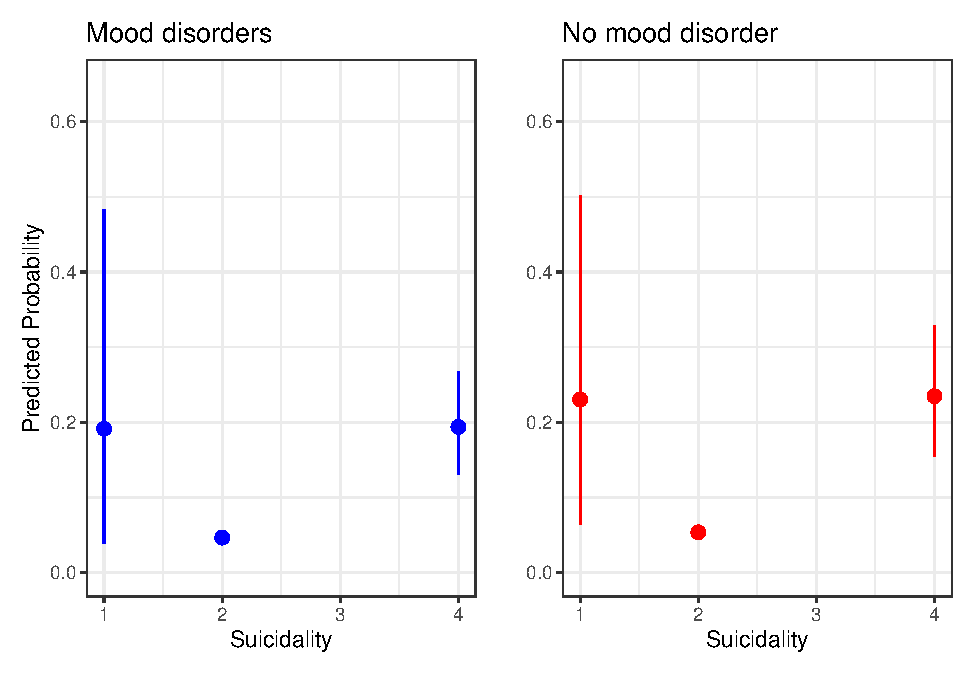
\includegraphics{MLE_3_files/figure-latex/graph-1.pdf}

There doesn't seem to be a difference between those with mood disorders
and those without (which is exactly what OLS told us). Let's look at the
results as a table.

\begin{Shaded}
\begin{Highlighting}[]
\FunctionTok{library}\NormalTok{(stargazer)}
\end{Highlighting}
\end{Shaded}

\begin{verbatim}
## 
## Please cite as:
\end{verbatim}

\begin{verbatim}
##  Hlavac, Marek (2018). stargazer: Well-Formatted Regression and Summary Statistics Tables.
\end{verbatim}

\begin{verbatim}
##  R package version 5.2.2. https://CRAN.R-project.org/package=stargazer
\end{verbatim}

\begin{Shaded}
\begin{Highlighting}[]
\NormalTok{star.out }\OtherTok{\textless{}{-}} \FunctionTok{stargazer}\NormalTok{(out1, ols)}
\end{Highlighting}
\end{Shaded}

\% Table created by stargazer v.5.2.2 by Marek Hlavac, Harvard
University. E-mail: hlavac at fas.harvard.edu \% Date and time: Sun, Jul
11, 2021 - 4:25:13 PM

\begin{table}[!htbp] \centering 
  \caption{} 
  \label{} 
\begin{tabular}{@{\extracolsep{5pt}}lcc} 
\\[-1.8ex]\hline 
\hline \\[-1.8ex] 
 & \multicolumn{2}{c}{\textit{Dependent variable:}} \\ 
\cline{2-3} 
\\[-1.8ex] & SISDB\_SUIC & SISDB\_SUIC \\ 
\\[-1.8ex] & \textit{ordered} & \textit{OLS} \\ 
 & \textit{logistic} & \textit{} \\ 
\\[-1.8ex] & (1) & (2)\\ 
\hline \\[-1.8ex] 
 SEX & $-$0.596$^{*}$ & $-$0.257$^{*}$ \\ 
  & (0.328) & (0.135) \\ 
  & & \\ 
 race & $-$1.038$^{***}$ & $-$0.445$^{***}$ \\ 
  & (0.388) & (0.166) \\ 
  & & \\ 
 SISDB\_SHARM & 1.314$^{***}$ & 0.553$^{***}$ \\ 
  & (0.164) & (0.055) \\ 
  & & \\ 
 SES & $-$0.003 & 0.001 \\ 
  & (0.009) & (0.004) \\ 
  & & \\ 
 MOODDX & 0.301 & 0.132 \\ 
  & (0.312) & (0.124) \\ 
  & & \\ 
 NEGLECT & $-$0.068 & $-$0.025 \\ 
  & (0.111) & (0.044) \\ 
  & & \\ 
 PASUM & 0.042 & 0.010 \\ 
  & (0.090) & (0.037) \\ 
  & & \\ 
 SCL\_PSY & 0.350$^{*}$ & 0.115 \\ 
  & (0.180) & (0.071) \\ 
  & & \\ 
 Constant &  & 1.283$^{***}$ \\ 
  &  & (0.326) \\ 
  & & \\ 
\hline \\[-1.8ex] 
Observations & 202 & 202 \\ 
R$^{2}$ &  & 0.497 \\ 
Adjusted R$^{2}$ &  & 0.476 \\ 
Residual Std. Error &  & 0.843 (df = 193) \\ 
F Statistic &  & 23.843$^{***}$ (df = 8; 193) \\ 
\hline 
\hline \\[-1.8ex] 
\textit{Note:}  & \multicolumn{2}{r}{$^{*}$p$<$0.1; $^{**}$p$<$0.05; $^{***}$p$<$0.01} \\ 
\end{tabular} 
\end{table}

\begin{Shaded}
\begin{Highlighting}[]
\NormalTok{star.out}
\end{Highlighting}
\end{Shaded}

{[}1{]} ""\\
{[}2{]} ``\% Table created by stargazer v.5.2.2 by Marek Hlavac, Harvard
University. E-mail: hlavac at fas.harvard.edu'' {[}3{]} ``\% Date and
time: Sun, Jul 11, 2021 - 4:25:13 PM''\\
{[}4{]} ``\textbackslash begin\{table\}{[}!htbp{]}
\textbackslash centering''\\
{[}5{]} " \textbackslash caption\{\} "\\
{[}6{]} " \textbackslash label\{\} "\\
{[}7{]}
``\textbackslash begin\{tabular\}\{@\{\textbackslash extracolsep\{5pt\}\}lcc\}''\\
{[}8{]}
``\textbackslash\textbackslash{[}-1.8ex{]}\textbackslash hline''\\
{[}9{]} ``\textbackslash hline
\textbackslash\textbackslash{[}-1.8ex{]}''\\
{[}10{]} " \&
\textbackslash multicolumn\{2\}\{c\}\{\textbackslash textit\{Dependent
variable:\}\} \textbackslash\textbackslash{} "\\
{[}11{]} ``\textbackslash cline\{2-3\}''\\
{[}12{]} "\textbackslash\textbackslash{[}-1.8ex{]} \&
SISDB\textbackslash\_SUIC \& SISDB\textbackslash\_SUIC
\textbackslash\textbackslash{} "\\
{[}13{]} ``\textbackslash\textbackslash{[}-1.8ex{]} \&
\textbackslash textit\{ordered\} \& \textbackslash textit\{OLS\}
\textbackslash\textbackslash{}''\\
{[}14{]} " \& \textbackslash textit\{logistic\} \&
\textbackslash textit\{\} \textbackslash\textbackslash{} "\\
{[}15{]} ``\textbackslash\textbackslash{[}-1.8ex{]} \& (1) \&
(2)\textbackslash\textbackslash{}''\\
{[}16{]} ``\textbackslash hline
\textbackslash\textbackslash{[}-1.8ex{]}''\\
{[}17{]} " SEX \& \$-\(0.596\)\^{}\{\emph{\}\$ \&
\$-\(0.257\)\^{}\{}\}\$ \textbackslash\textbackslash{} "\\
{[}18{]} " \& (0.328) \& (0.135) \textbackslash\textbackslash{} "\\
{[}19{]} " \& \& \textbackslash\textbackslash{} "\\
{[}20{]} " race \& \$-\(1.038\)\^{}\{\textbf{\emph{\}\$ \&
\$-\(0.445\)\^{}\{}}\}\$ \textbackslash\textbackslash{} "\\
{[}21{]} " \& (0.388) \& (0.166) \textbackslash\textbackslash{} "\\
{[}22{]} " \& \& \textbackslash\textbackslash{} "\\
{[}23{]} " SISDB\textbackslash\_SHARM \& 1.314\(^{***}\) \&
0.553\(^{***}\) \textbackslash\textbackslash{} "\\
{[}24{]} " \& (0.164) \& (0.055) \textbackslash\textbackslash{} "\\
{[}25{]} " \& \& \textbackslash\textbackslash{} "\\
{[}26{]} " SES \& \$-\$0.003 \& 0.001 \textbackslash\textbackslash{} "\\
{[}27{]} " \& (0.009) \& (0.004) \textbackslash\textbackslash{} "\\
{[}28{]} " \& \& \textbackslash\textbackslash{} "\\
{[}29{]} " MOODDX \& 0.301 \& 0.132 \textbackslash\textbackslash{} "\\
{[}30{]} " \& (0.312) \& (0.124) \textbackslash\textbackslash{} "\\
{[}31{]} " \& \& \textbackslash\textbackslash{} "\\
{[}32{]} " NEGLECT \& \$-\$0.068 \&
\$-\(0.025 \\\\ " [33] " & (0.111) & (0.044) \\\\ " [34] " & & \\\\ " [35] " PASUM & 0.042 & 0.010 \\\\ " [36] " & (0.090) & (0.037) \\\\ " [37] " & & \\\\ " [38] " SCL\\_PSY & 0.350\)\^{}\{*\}\$
\& 0.115 \textbackslash\textbackslash{} "\\
{[}39{]} " \& (0.180) \& (0.071) \textbackslash\textbackslash{} "\\
{[}40{]} " \& \& \textbackslash\textbackslash{} "\\
{[}41{]} " Constant \& \& 1.283\(^{***}\) \textbackslash\textbackslash{}
"\\
{[}42{]} " \& \& (0.326) \textbackslash\textbackslash{} "\\
{[}43{]} " \& \& \textbackslash\textbackslash{} "\\
{[}44{]} ``\textbackslash hline
\textbackslash\textbackslash{[}-1.8ex{]}''\\
{[}45{]} ``Observations \& 202 \& 202 \textbackslash\textbackslash{}''\\
{[}46{]} ``R\(^{2}\) \& \& 0.497 \textbackslash\textbackslash{}''\\
{[}47{]} ``Adjusted R\(^{2}\) \& \& 0.476
\textbackslash\textbackslash{}''\\
{[}48{]} ``Residual Std. Error \& \& 0.843 (df = 193)
\textbackslash\textbackslash{}''\\
{[}49{]} ``F Statistic \& \& 23.843\(^{***}\) (df = 8; 193)
\textbackslash\textbackslash{}''\\
{[}50{]} ``\textbackslash hline''\\
{[}51{]} ``\textbackslash hline
\textbackslash\textbackslash{[}-1.8ex{]}''\\
{[}52{]} ``\textbackslash textit\{Note:\} \&
\textbackslash multicolumn\{2\}\{r\}\{\(^{*}\)p\$\textless\$0.1;
\(^{**}\)p\$\textless\$0.05; \(^{***}\)p\$\textless\$0.01\}
\textbackslash\textbackslash{}''\\
{[}53{]} ``\textbackslash end\{tabular\}''\\
{[}54{]} ``\textbackslash end\{table\}''

\end{document}
